%%%%%%%%%%%%%%%%%%%%%%%%%%%%%%%%%%%%%%%%%%%%%%%%%%%%%%%%%%%%%%%%%%%%%%%%%%%%%%%%%%
\begin{frame}[fragile]\frametitle{}
\begin{center}
{\Large Vertex AI RAG Engine}

{\tiny (Ref: https://cloud.google.com/vertex-ai/generative-ai/docs/rag-engine/rag-overview)}
\end{center}
\end{frame}

%%%%%%%%%%%%%%%%%%%%%%%%%%%%%%%%%%%%%%%%%%%%%%%%%%%%%%%%%%%
\begin{frame}[fragile]\frametitle{Vertex AI RAG Engine: Introduction}
      \begin{itemize}
        \item Component of Vertex AI Platform facilitating Retrieval-Augmented Generation
        \item Data framework for developing context-augmented LLM applications
        \item Addresses common LLM limitation: lack of knowledge about private organizational data
        \item Enriches LLM context with additional private information
        \item Reduces hallucination and improves answer accuracy
        \item Combines external knowledge sources with LLM's existing knowledge
      \end{itemize}
\end{frame}

%%%%%%%%%%%%%%%%%%%%%%%%%%%%%%%%%%%%%%%%%%%%%%%%%%%%%%%%%%%
\begin{frame}[fragile]\frametitle{RAG Process Overview}
      \begin{itemize}
        \item Data Ingestion: Intake from various sources (local files, Cloud Storage, Google Drive)
        \item Data Transformation: Convert and prepare data for indexing (chunking)
        \item Embedding: Create numerical representations capturing semantic meaning
        \item Data Indexing: Create a corpus optimized for searching
        \item Retrieval: Find relevant information based on user queries
        \item Generation: Use retrieved context with user query for informed responses
      \end{itemize}
\end{frame}

%%%%%%%%%%%%%%%%%%%%%%%%%%%%%%%%%%%%%%%%%%%%%%%%%%%%%%%%%%%
\begin{frame}[fragile]\frametitle{RAG Process Overview}

\begin{center}
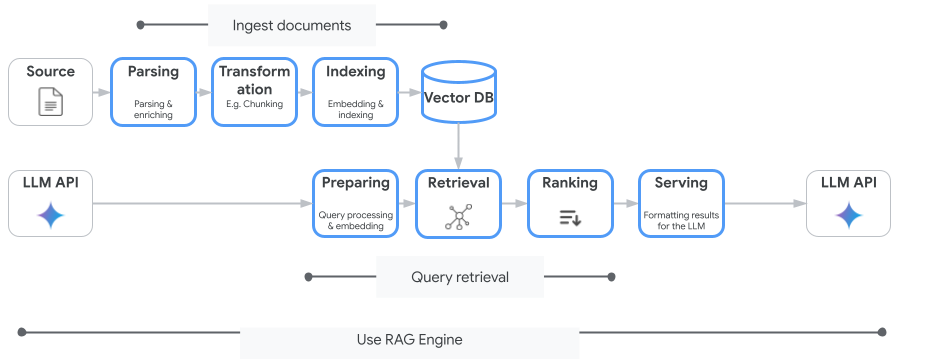
\includegraphics[width=\linewidth,keepaspectratio]{rag37}
\end{center}	
\end{frame}


%%%%%%%%%%%%%%%%%%%%%%%%%%%%%%%%%%%%%%%%%%%%%%%%%%%%%%%%%%%
\begin{frame}[fragile]\frametitle{Benefits of Vertex AI RAG Engine}
      \begin{itemize}
        \item Provides factual grounding for LLM responses
        \item Allows integration of proprietary/private data
        \item Improves response accuracy and relevance
        \item Reduces LLM hallucinations
        \item Creates domain-specific AI applications
        \item Enables knowledge-based conversational experiences
      \end{itemize}
\end{frame}


%%%%%%%%%%%%%%%%%%%%%%%%%%%%%%%%%%%%%%%%%%%%%%%%%%%%%%%%%%%
\begin{frame}[fragile]\frametitle{Getting Started with Vertex AI RAG}
      \begin{itemize}
        \item Create a new GCP Project (console.cloud.google.com)
        \item Enable the Vertex AI API
        \item Install Vertex AI SDK for Python
        \item Set up project authentication
      \end{itemize}
	  
\begin{lstlisting}[language=bash]
pip install google-cloud-aiplatform

gcloud config set {project}
gcloud auth application-default login
\end{lstlisting}	  
\end{frame}

%%%%%%%%%%%%%%%%%%%%%%%%%%%%%%%%%%%%%%%%%%%%%%%%%%%%%%%%%%%
\begin{frame}[fragile]\frametitle{Python SDK Imports (Example)}
    \begin{lstlisting}[language=python]
import vertexai
from google.cloud.aiplatform.private_preview import rag
from vertexai.generative_models import GenerativeModel, Tool

# PROJECT_ID = "your-google-cloud-project-id"
# REGION = "us-central1" # Or your preferred region
# CORPUS_DISPLAY_NAME = "my_rag_corpus"
# GCS_BUCKET_NAME = "your-gcs-bucket-for-rag-docs"
# EMBEDDING_MODEL_PUBLISHER_PATH = "publishers/google/models/textembedding-gecko@003" # Verify model

# vertexai.init(project=PROJECT_ID, location=REGION)
    \end{lstlisting}
\end{frame}


%%%%%%%%%%%%%%%%%%%%%%%%%%%%%%%%%%%%%%%%%%%%%%%%%%%%%%%%%%%
\begin{frame}[fragile]\frametitle{Creating a RAG Corpus}
      \begin{itemize}
        \item Initialize Vertex AI and configure embedding model
        \item Create a RAG corpus with appropriate configuration
      \end{itemize}
		
        \begin{lstlisting}[language=python]
vertexai.init(project=PROJECT_ID, location="us-central1")

embedding_model_config = rag.RagEmbeddingModelConfig(
    vertex_prediction_endpoint=rag.VertexPredictionEndpoint(
        publisher_model="publishers/google/models/text-embedding-005"
    )
)

rag_corpus = rag.create_corpus(
    display_name=display_name,
    backend_config=rag.RagVectorDbConfig(
        rag_embedding_model_config=embedding_model_config
    ),
)
        \end{lstlisting}
\end{frame}

%%%%%%%%%%%%%%%%%%%%%%%%%%%%%%%%%%%%%%%%%%%%%%%%%%%%%%%%%%%
\begin{frame}[fragile]\frametitle{Importing Files to RAG Corpus}
      \begin{itemize}
        \item Import documents from Google Cloud Storage or Google Drive
        \item Configure chunking parameters for optimal retrieval
      \end{itemize}
		
        \begin{lstlisting}[language=python]
rag.import_files(
    rag_corpus.name,
    paths,  # GCS or Google Drive paths
    transformation_config=rag.TransformationConfig(
        chunking_config=rag.ChunkingConfig(
            chunk_size=512,
            chunk_overlap=100,
        ),
    ),
    max_embedding_requests_per_min=1000,  # Optional
)
        \end{lstlisting}
\end{frame}

%%%%%%%%%%%%%%%%%%%%%%%%%%%%%%%%%%%%%%%%%%%%%%%%%%%%%%%%%%%
\begin{frame}[fragile]\frametitle{Direct Context Retrieval}
      \begin{itemize}
        \item Configure retrieval parameters (top-k results, relevance filters)
        \item Query corpus directly for relevant context
      \end{itemize}
		
        \begin{lstlisting}[language=python]
rag_retrieval_config = rag.RagRetrievalConfig(
    top_k=3,  # Optional
    filter=rag.Filter(vector_distance_threshold=0.5),
)
response = rag.retrieval_query(
    rag_resources=[
        rag.RagResource(
            rag_corpus=rag_corpus.name,
            # Optional: specific file IDs
        )
    ],
    text="What is RAG and why it is helpful?",
    rag_retrieval_config=rag_retrieval_config,
)
print(response)
        \end{lstlisting}
\end{frame}

%%%%%%%%%%%%%%%%%%%%%%%%%%%%%%%%%%%%%%%%%%%%%%%%%%%%%%%%%%%
\begin{frame}[fragile]\frametitle{Enhancing LLM Generation with RAG}
      \begin{itemize}
        \item Create a RAG retrieval tool for the LLM
        \item Initialize Gemini model with the retrieval tool
        \item Generate augmented responses
      \end{itemize}
		
      \begin{lstlisting}[language=python]
rag_retrieval_tool = Tool.from_retrieval(
    retrieval=rag.Retrieval(
        source=rag.VertexRagStore(
            rag_resources=[rag.RagResource(rag_corpus=rag_corpus.name,)],
            rag_retrieval_config=rag_retrieval_config,),))

rag_model = GenerativeModel( model_name="gemini-2.0-flash-001", 
    tools=[rag_retrieval_tool])

response = rag_model.generate_content(
    "What is RAG and why it is helpful?")
print(response.text)
      \end{lstlisting}
\end{frame}

%%%%%%%%%%%%%%%%%%%%%%%%%%%%%%%%%%%%%%%%%%%%%%%%%%%%%%%%%%%
\begin{frame}[fragile]\frametitle{Advanced RAG Capabilities}
      \begin{itemize}
        \item Filter retrieval by specific document IDs
        \item Adjust vector distance thresholds for relevance
        \item Configure chunking parameters for optimal retrieval
        \item Scale with configurable embedding request rates
        \item Support for multiple document formats and sources
        \item Integration with other Vertex AI capabilities
      \end{itemize}
\end{frame}

%%%%%%%%%%%%%%%%%%%%%%%%%%%%%%%%%%%%%%%%%%%%%%%%%%%%%%%%%%%
\begin{frame}[fragile]\frametitle{Best Practices}
      \begin{itemize}
        \item Optimize chunk size for your specific content
        \item Balance chunk overlap for contextual coherence
        \item Tune top-k and relevance thresholds for your use case
        \item Consider multiple corpora for different knowledge domains
        \item Test queries against your corpus before deployment
        \item Monitor and refine based on generation quality
      \end{itemize}
\end{frame}